\documentclass[a4paper, 12pt]{article}
\usepackage[utf8]{inputenc}
\usepackage[spanish]{babel}
\usepackage{geometry}
\geometry{left=3cm, right=3cm, top=3cm, bottom=3cm}
\usepackage{graphicx}
\usepackage{hyperref}
\usepackage{titlesec}
\usepackage{fancyhdr}
\usepackage{natbib}
\bibliographystyle{plain}

% Encabezado y pie de página
\pagestyle{fancy}
\fancyhf{}
\lhead{\university}
\rhead{\faculty}
\cfoot{\thepage}
% Figura entre los nombres y la universidad

% Formato de secciones
\titleformat{\section}{\normalfont\Large\bfseries}{\thesection}{1em}{}
\titleformat{\subsection}{\normalfont\large\bfseries}{\thesubsection}{1em}{}

% Título del informe
\title{\textbf{La Automatización del Ajedrez DeepBlue} \\ \subtitle}
\author{Daniel Machado Pérez \\ Ariel González Gómez}

\newcommand{\subtitle}{\textit{Historia de la Computación}}
\newcommand{\university}{Universidad de La Habana}
\newcommand{\faculty}{Facultad de Matemática y Computación}
\newcommand{\githubrepo}{\href{https://github.com/DanielMPMatCom/Historia-de-la-Computacion.-DeepBlue.git}{Repositorio en GitHub}}

\begin{document}

% Encabezado con imágenes
\begin{figure}[t]
    
\includegraphics[width=0.15\textwidth]{assets/UH.jpg}
    \hfill
    
\includegraphics[width=0.2\textwidth]{assets/MatCom sin fondo color.png}
\end{figure}
\vspace{-2cm}

% Título principal
\maketitle

% Figura entre nombres y universidad
\begin{figure}[h!]
    \centering
    
\includegraphics[width=0.3\textwidth]{assets/logo.jpg}
\end{figure}

% Información adicional
\begin{center}
    \large \university \\
    \faculty \\
    \vspace{3.5cm}
    \githubrepo
\end{center}
\newpage
\tableofcontents
\newpage

% Resumen

\begin{abstract}
    El presente informe analiza en detalle la evolución y los 
    componentes técnicos de \textit{Deep Blue}, la primera 
    máquina capaz de derrotar al campeón mundial de ajedrez 
    bajo condiciones reglamentarias. Se describen los 
    antecedentes desde ChipTest y Deep Thought, la arquitectura 
    de hardware VLSI y del clúster IBM RS/6000 SP, los 
    algoritmos de búsqueda híbrida en C con créditos diferidos y 
    la función de evaluación implementada en silicio. Además, 
    se examinan los mecanismos de paralelismo y balance de carga, 
    el soporte de libros de aperturas y bases de finales, así 
    como las estrategias de control de tiempo. Finalmente, se 
    evalúa el impacto histórico y el legado de \textit{Deep Blue} 
    en la supercomputación y la inteligencia artificial aplicada, 
    destacando su papel en el paso de enfoques de fuerza bruta a 
    sistemas híbridos con conocimiento experto.
\end{abstract}
    

\newpage
% region Introducción
% Introducción
\section{Introducción}

Desde sus inicios, el juego de ajedrez ha sido considerado un 
terreno fértil para evaluar la capacidad de las máquinas para 
replicar formas avanzadas de pensamiento humano. La complejidad 
combinatoria del ajedrez, junto con su estructura formal y 
reglas bien definidas, lo convierten en un banco de pruebas 
ideal para los sistemas de inteligencia artificial. En este 
contexto, el desarrollo de \textit{Deep Blue} por parte de IBM 
representa un hito en la historia de la computación, no solo por 
su impacto mediático, sino también por los avances técnicos y 
conceptuales que introdujo en la automatización del razonamiento 
estratégico.

\textit{Deep Blue} no fue un simple programa de ajedrez, sino un 
sistema computacional altamente especializado que integraba 
componentes de hardware diseñados específicamente para el 
cálculo masivo de posiciones y movimientos posibles, junto con 
sofisticados algoritmos de búsqueda y evaluación posicional. La 
arquitectura del sistema combinó miles de procesadores en 
paralelo con chips dedicados a operaciones de ajedrez, 
permitiendo una profundidad de búsqueda y una velocidad de 
procesamiento inalcanzables para cualquier computadora 
convencional de su época.

Más allá de su capacidad para vencer a un campeón mundial, lo 
que convierte a \textit{Deep Blue} en un objeto de estudio 
técnico relevante es su enfoque híbrido de solución: una 
articulación precisa entre potencia de cálculo, paralelismo 
masivo y conocimiento experto codificado. Este informe se centra 
en analizar los componentes técnicos que hicieron posible dicha 
hazaña, incluyendo tanto los aspectos de hardware como los 
mecanismos algorítmicos empleados, y cómo estos interactúan de 
forma coordinada para lograr un rendimiento sobresaliente en la 
resolución de un problema complejo como el ajedrez.

El objetivo de este estudio no es explorar los aspectos 
históricos del enfrentamiento entre \textit{Deep Blue} y Garry 
Kasparov, aunque se comentará brevemente su contexto; el foco 
principal recae sobre los elementos estructurales y funcionales 
del sistema, desde su arquitectura paralela hasta las 
heurísticas que guían la evaluación de posiciones. A través de 
este análisis técnico, se busca comprender cómo la integración 
eficaz de recursos computacionales puede acercarse, e incluso 
superar, ciertas formas de cognición humana en dominios bien 
estructurados.


\newpage
% region Desarrollo
% Desarrollo


\section{Antecedentes del ajedrez computacional. De ChipTest a Deep Thought}

\subsection{ChipTest}
El proyecto ChipTest se inició en 1985 en la Universidad 
Carnegie Mellon bajo la dirección de Feng-hsiung Hsu, Thomas 
Anantharaman y Murray Campbell, con el objetivo de explorar la 
viabilidad de un generador de movimientos de ajedrez 
implementado en VLSI \cite{Hsu1988}. La primera versión de 
ChipTest estaba controlada por una estación de trabajo 
Sun-3/160 y alcanzaba aproximadamente 50000 posiciones por 
segundo \cite{Hsu1988}. En 1986, ChipTest compitió en el North 
American Computer Chess Championship, donde, pese a contar con 
pruebas limitadas antes del torneo, consiguió recuperarse tras 
un inicio adverso y obtuvo un resultado equilibrado 
\cite{Hsu1988}.

\subsection{ChipTest-M y transición a Deep Thought}
En agosto de 1987 se rediseñó ChipTest y se rebautizó como 
ChipTest-M, multiplicando por diez su velocidad de búsqueda 
hasta alrededor de 500000 posiciones por segundo, ya sobre una 
Sun-4 \cite{Hsu1989}. Esta versión se alzó con el título en el 
NACCC de 1987 con un marcador de 4-0 \cite{Hsu1989}. El éxito de 
ChipTest-M condujo al desarrollo de Deep Thought: la versión 
0.01 apareció en mayo de 1988 y la 0.02 en noviembre del mismo 
año, incorporando dos procesadores VLSI dedicados y elevando la 
tasa de búsqueda a casi 700000 posiciones por segundo 
\cite{Hsu1990}. Con Deep Thought, el equipo obtuvo el título en 
el World Computer Chess Championship de 1989 con un resultado 
perfecto de 5-0 \cite{Hsu1990}.

\subsection{Primeros éxitos y limitaciones}

Deep Thought destacó en 1988 al compartir el primer puesto en el 
Software Toolworks Open de Los Ángeles, donde venció al gran 
maestro Bent Larsen, consiguiendo una valoración de rendimiento 
(USCF) de 2551 y ganando el Fredkin Intermediate Prize 
\cite{Hsu1990}. Asimismo, ganó el ACM Computer Chess 
Championship en Orlando ese mismo año \cite{Hsu1990}. Pese a 
estos logros, la arquitectura de ChipTest y Deep Thought 
permanecía limitada por un grado de paralelismo moderado 
(dos chips VLSI en configuración típico o procesadores 
uniprocesador), lo que restringía la profundidad uniforme de 
búsqueda y obligaba a depender intensamente de heurísticas de 
selección y extensiones locales para obtener rendimiento 
competitivo \cite{Hsu1990}.








\section{Origen y maduración de Deep Blue}

\subsection{Incorporación a IBM y renombrado}

A finales de 1989, parte del equipo original de ChipTest y Deep 
Thought (Feng-hsiung Hsu y Murray Campbell) pasó al IBM T.J. 
Watson Research Center para continuar el desarrollo de máquinas 
de ajedrez de alto rendimiento. En este nuevo entorno se 
estableció el proyecto \textit{Deep Thought 2}, considerado el 
paso intermedio hacia lo que pronto sería conocido como 
\textit{Deep Blue} \cite{Campbell2002}. Bajo la dirección de la 
división de investigación de IBM, el sistema heredó la 
arquitectura basada en chips VLSI especializada para generar y 
evaluar movimientos de ajedrez, al tiempo que incorporaba 
herramientas de software más avanzadas para depuración, 
afinamiento de la función de evaluación y análisis de partidas 
\cite{Campbell2002}.

\begin{figure}[h]
    \centering
    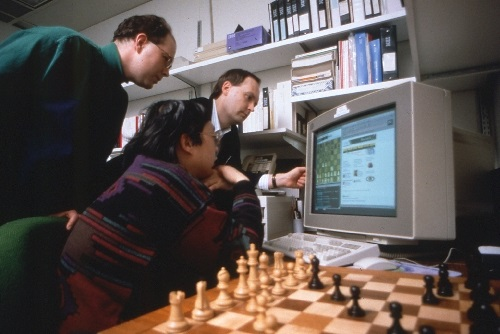
\includegraphics[width=0.6\textwidth]{assets/Deep Blue's core team, Joe Hoane, Feng-hsiung Hsu, and Murray Campbell.jpg}
    \caption{Equipo central de Deep Blue, Joe Hoane, Feng-hsiung Hsu y Murray Campbell.}
    \label{fig:team}
\end{figure}


\subsection{Deep Blue I (1995-1996)}

El prototipo \textit{Deep Blue I} comenzó a tomar forma en 1995, 
tras tres años de diseño de un chip de búsqueda único. La 
primera remesa de circuitos llegó en septiembre de ese año y, 
una vez solucionados los defectos iniciales, en enero de 1996 se 
dispuso de la versión estable. El sistema corría sobre un 
clúster IBM RS/6000 SP de 36 nodos y empleaba 216 chips VLSI, 
cada uno capaz de explorar entre 1.6 y 2 millones de posiciones 
por segundo. En conjunto, la máquina alcanzaba velocidades de 
entre 50 y 100 millones de posiciones por segundo \cite{Campbell2002}.    

En febrero de 1996, \textit{Deep Blue I} se enfrentó a Garry 
Kasparov bajo condiciones de torneo: tras empatar 2-2 en las 
cuatro primeras partidas, Kasparov ganó los dos encuentros 
finales, venciendo por 4-2 \cite{Campbell2002}. Aunque el 
resultado favoreció al campeón humano, la serie demostró que una 
máquina especialmente diseñada podía competir de tú a tú con la 
élite mundial.

\subsection{Deep Blue II (1996-1997)}

Tras el match de 1996 quedó patente la necesidad de mejorar la 
función de evaluación y aumentar el paralelismo. En respuesta, 
IBM diseñó un nuevo chip que amplió los rasgos de evaluación de 
alrededor de 6 400 a más de 8 000, incorporó detección de 
repeticiones en hardware y optimizaciones en generación de 
jugadas, elevando la velocidad de cada chip a 2-2.5 millones de 
posiciones por segundo. Además, el sistema pasó a disponer de 
480 chips VLSI distribuidos en 30 nodos SP, duplicando con 
creces la capacidad de búsqueda \cite{Campbell2002}.

Entre enero y mayo de 1997, el equipo dedicó la mayor parte de 
sus esfuerzos a afinar la función de evaluación y a preparar la 
base de datos de aperturas y finales. El resultado fue 
\textit{Deep Blue II}, que derrotó a Kasparov por 3\(\frac{1}{2}\)-2\(\frac{1}{2}\) en mayo
de 1997, convirtiéndose en la primera máquina en vencer al 
campeón mundial en un match reglamentario y recibiendo por 
ello el Premio Fredkin \cite{Campbell2002}.



\begin{figure}[h]
    \centering
    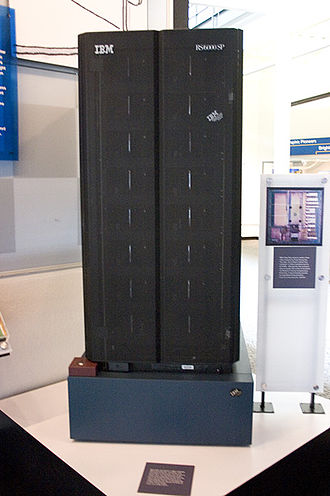
\includegraphics[width=0.6\textwidth]{assets/deepblue.jpg}
    \caption{Deep Blue.}
    \label{fig:deepblue}
\end{figure}










\section{Arquitectura del sistema}

\subsection{Infraestructura IBM RS/6000 SP}

El corazón de \textit{Deep Blue} es un clúster IBM RS/6000 SP 
compuesto por treinta nodos equipados con procesadores Power2 
Super Chip (P2SC), de los cuales veintiocho funcionan a una 
frecuencia de 120 MHz y dos a 135 MHz. Cada nodo dispone de 1 GB 
de memoria RAM y 4 GB de almacenamiento local. La interconexión 
se realiza mediante un conmutador de alta velocidad que 
implementa el estándar MPI, garantizando una latencia mínima en 
el envío y recepción de posiciones de ajedrez durante la 
búsqueda paralela \cite{Campbell2002, hsu1999ibm}.

\subsection{Chips especializados}

Para alcanzar velocidades de exploración de árbol imposibles en 
un ordenador convencional, \textit{Deep Blue} emplea 480 chips 
VLSI especializados, distribuidos en los treinta nodos SP. Cada 
chip integra tres módulos fundamentales: un generador de 
movimientos basado en lógica combinatoria (matriz 8x8), una 
función de evaluación en dos niveles —rápida (un ciclo de reloj) 
y lenta (análisis columna por columna de estructuras complejas)—, 
y un controlador de búsqueda alpha-beta de ventana nula con 
extensiones locales (jaques, peones pasados, detección de 
repeticiones en 32 plies) \cite{Campbell2002}. Este diseño en 
silicio permite examinar, de forma acumulada, entre 2 y 2.5 
millones de posiciones por segundo por chip. \cite{hsu1999ibm}

\begin{figure}[h]
    \centering
    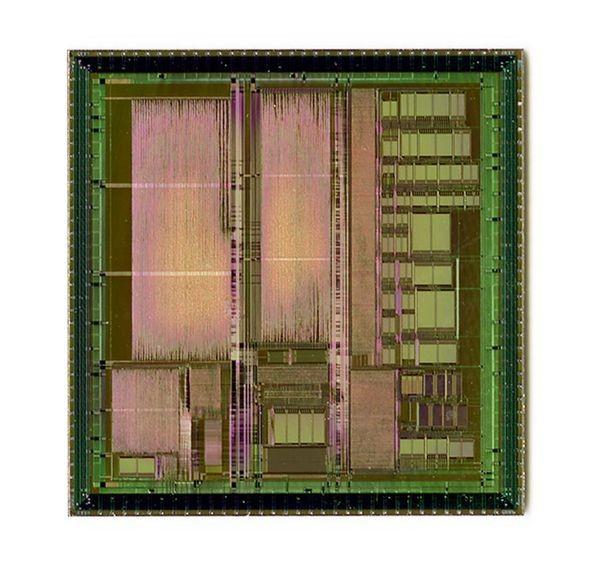
\includegraphics[width=0.6\textwidth]{assets/deep-blue-chip.jpg}
    \caption{Esquema del chip VLSI de Deep Blue: generador de movimientos, evaluación rápida/lenta y controlador alpha-beta de ventana nula.}
    \label{fig:chip_vlsi}
\end{figure}

\subsection{Jerarquía Maestro--Trabajador--Chip}


La ejecución de la búsqueda se organiza jerárquicamente en tres 
niveles. En el nivel superior, un nodo maestro realiza las 
primeras iteraciones de la búsqueda, generando posiciones 
“hoja” de tamaño medio. A continuación, esos nodos hoja se 
distribuyen entre veintinueve nodos trabajadores que profundizan 
el análisis unas pocas plies más, aplicando tablas de 
transposición y heurísticas de selección. Finalmente, cada 
trabajador delega las posiciones finales a un grupo de chips 
VLSI (16 por nodo) para que efectúen la búsqueda más profunda y 
quiescente en hardware. Esta arquitectura maestro-trabajador-chip 
maximiza el paralelismo y mantiene siempre ocupados tanto los 
procesadores como los chips especializados \cite{Campbell2002, hsu1999ibm}.










\section{Algoritmos de búsqueda y evaluación}

La fortaleza de \textit{Deep Blue} radica en la combinación 
sinérgica de un motor de búsqueda en software con una evaluación 
especializada en hardware. Este enfoque híbrido permite 
explotar al máximo tanto la flexibilidad algorítmica como la 
velocidad de procesamiento en silicio \cite{campbell1999search}.

\subsection{Búsqueda selectiva híbrida}

El motor en C emplea el algoritmo “dual credit with delayed 
extensions”, que otorga \emph{créditos} parciales a movimientos 
forzantes o de elevado carácter táctico (FFP) y sólo los 
\emph{canjea} cuando su acumulación supera un umbral predefinido, 
evitando así explosiones en la exploración del árbol de juego. 
Para preservar la coherencia de la 
Variación Principal, cada bando mantiene su propia cuenta de 
crédito y, al extenderse uno, se descuenta el mismo importe al 
adversario, garantizando un “sobre de búsqueda” que impide 
re-búsquedas oscilantes. Gracias a este 
mecanismo, \textit{Deep Blue} ajusta dinámicamente la 
profundidad de búsqueda en función de la complejidad táctica de 
la posición, llegando a profundidades efectivas de hasta 
cuarenta plies en las variantes más forzadas \cite{campbell1999search}.

\subsection{Evaluación en hardware}

La evaluación de posiciones se realiza completamente en 
silicio mediante más de 8 000 patrones VLSI. En un primer paso, 
la evaluación rápida suma en un único ciclo de reloj los valores 
básicos de material y posicionamiento. A continuación, la 
evaluación lenta analiza columna por columna estructuras 
posicionales complejas —como seguridad de rey, configuración de 
peones y control de casillas críticas— utilizando tablas 
parametrizables cuyos pesos fueron ajustados por herramientas 
automáticas y entrenamiento comparativo. Este diseño asegura que cada 
evaluación se ejecute en tiempo constante, sin degradar la 
velocidad global de búsqueda \cite{campbell1999search}.

\subsection{Extensiones y búsqueda cuiescente}

Para mitigar el “efecto horizonte” y capturar tácticas 
decisivas, \textit{Deep Blue} aplica extensiones locales y 
búsqueda cuiescente tanto en hardware como en software. 
Entre los criterios de extensión destacan la \emph{singularidad} 
(cuando un movimiento es claramente superior a todas las alternativas, 
se extiende 1-2 plies adicionales) y los \emph{chequeos} o 
\emph{empuje de peón a séptima}, que reciben tratamiento 
preferente para explorar líneas forzadas. 
La detección de repeticiones se implementa mediante un buffer 
circular de 32 plies en el chip, que invalida automáticamente 
ramas cíclicas mediante un fallo bajo (“fail-low”) \cite{campbell1999search}.  

La búsqueda cuiescente continúa hasta que no quedan capturas 
críticas ni amenazas inmediatas, garantizando que sólo se 
evalúen posiciones \emph{quietas} y evitando así que variantes 
tácticas escapadas distorsionen la valoración final.














\section{Paralelismo y rendimiento}

\subsection{Paralelismo en software}

El paralelismo en software de \textit{Deep Blue} se articula en 
varios niveles para maximizar el aprovechamiento de los 30 
nodos SP antes de delegar en hardware. En primer lugar, se 
emplea \emph{PV-parallelism}, donde tras explorar el primer 
movimiento de la Variación Principal (PV) todas las alternativas 
pueden evaluarse en paralelo con ventanas de búsqueda 
desplazadas para conservar la selectividad \cite{Campbell2002}. 
En segundo lugar, en nodos que “fallan alto” (fail-high), se 
pueden lanzar en paralelo búsquedas de profundidad reducida 
para refinar amenazas y extensiones, mientras que en nodos que 
“fallan bajo” (fail-low) todas las ramas se procesan 
concurrentemente hasta encontrar un corte \cite{Campbell2002}. 
Finalmente, la sincronización global se realiza al término de 
cada iteración de búsqueda, garantizando consistencia de las 
tablas de transposición y de los datos de análisis antes de 
pasar a la siguiente profundidad \cite{Campbell2002}.

\subsection{Offloading a hardware}

Una vez exploradas varias capas en software, \textit{Deep Blue} 
\emph{offloads} de forma asíncrona las posiciones finales a los 
480 chips VLSI. Cada nodo SP puede gestionar múltiples búsquedas 
de chip en paralelo, enviando trabajos y recibiendo resultados 
sin bloquearse en espera de la finalización de cada tarea 
\cite{Campbell2002}. Para mantener un balance de carga 
adecuado, las búsquedas en hardware que exceden las 8000 
posiciones expandidas pueden abortarse y reencolarse en 
software, permitiendo dividirlas en subproblemas más pequeños y 
redistribuirlos entre otros nodos SP \cite{Campbell2002}.

\subsection{Medición de eficiencia}

Los experimentos de rendimiento con una configuración de un solo 
nodo SP (24 chips) mostraron eficiencias del 75\% en posiciones 
relativamente quietas y del 30\% en aquellas con tácticas 
profundas, reflejando la capacidad de paralelizar ramas 
homogéneas y de adaptarse a nodos muy desequilibrados 
\cite{Campbell2002}. Al escalar al sistema completo de 30 nodos, 
se estimó una eficiencia global de aproximadamente 12\% en 
posiciones tranquilas y 8\% en posiciones tácticas, debido 
principalmente a la sobrecarga de comunicación y a la 
variabilidad en el tamaño de las subramas \cite{Campbell2002}.




















\section{Componentes de apoyo}

\subsection{Libro de aperturas}

El libro de aperturas de \textit{Deep Blue} fue ensamblado 
manualmente por el Gran Maestro Joel Benjamin, junto con los 
Grandmasters Nick De Firmian, John Fedorowicz y Miguel Illescas, 
y contenía aproximadamente 4 000 posiciones seleccionadas según 
la experiencia práctica del sistema \cite{Campbell2002}. Cada 
posición del libro fue comprobada mediante ejecuciones nocturnas 
de \textit{Deep Blue} para asegurar que las líneas propuestas 
resultaran razonables bajo el motor de búsqueda, priorizando 
aquellas aperturas en las que el sistema demostraba mayor 
robustez táctica \cite{Campbell2002}. Antes de cada encuentro, 
se elegía un repertorio específico en función de la situación 
del match y de la elección de color, incluyéndose un pequeño 
“override book” de última hora para correcciones de último 
minuto \cite{Campbell2002}.

\subsection{Extended Book}

Cuando una posición no estaba cubierta por el libro principal, 
\textit{Deep Blue} empleaba un “libro extendido” basado en un 
repositorio de cerca de 700 000 partidas de Grandes Maestros 
\cite{Campbell2002}. A cada jugada candidateada se le asignaba 
una bonificación escalar calculada a partir de la frecuencia de 
aparición en la base de datos, la fuerza de los jugadores que la 
emplearon, los resultados estadísticos y las anotaciones 
(marcas “!” o “?”), de manera no lineal y ponderada para 
reflejar consenso teórico de apertura \cite{Campbell2002}. 
En situaciones extremas, una bonificación superior a medio 
peón permitía ejecutar la jugada directamente sin activación de 
la búsqueda completa \cite{Campbell2002}.

\subsection{Bases de datos de finales}

Para los finales, \textit{Deep Blue} recurría a bases de datos 
de finales con todas las posiciones de hasta cinco piezas y 
casos seleccionados de seis piezas (por ejemplo, peones 
bloqueados), extraídas principalmente de Colecciones de Ken 
Thompson y contribuciones de Lewis Stiller \cite{Campbell2002}. 
Cada posición se indexaba como un bit (ganar o no perder), de 
modo que al alcanzarse durante la búsqueda se aplicaba 
inmediatamente un \emph{cutoff} con valor teórico—alto orden 
para la victoria o empate, bajo orden para el desempate según 
evaluación estática—sin necesidad de desarrollar subárboles 
adicionales \cite{Campbell2002}. Estas bases residían localmente 
en cada nodo SP y en arreglos RAID compartidos, garantizando 
acceso rápido en tiempo de búsqueda \cite{Campbell2002}.

\subsection{Control de tiempo}

El mecanismo de control de tiempo de \textit{Deep Blue} definía 
dos objetivos temporales antes de cada movida: un tiempo 
“normal”, calculado como el tiempo restante hasta el próximo 
control dividido por los movimientos estimados, y un tiempo 
“pánico” equivalente a un tercio del tiempo restante 
\cite{Campbell2002}. Si al alcanzar el tiempo normal no se 
detectaban condiciones excepcionales, el sistema jugaba el mejor 
movimiento disponible; en caso de variación excesiva en el valor 
del movimiento (más de 15 centipawns) o estados de 
\emph{fail-low/high}, la búsqueda continuaba hasta nueva 
resolución o hasta el tiempo pánico, circunstancia que solo 
ocurrió una vez en todo el match de 1997 \cite{Campbell2002}.















\section{Impacto y legado}

\subsection{Hito en IA y supercomputación}

En mayo de 1997, \textit{Deep Blue} se convirtió en el primer 
sistema informático capaz de derrotar a un campeón mundial de 
ajedrez bajo condiciones reglamentarias de torneo, venciendo a 
Garry Kasparov por 3\(\frac{1}{2}\)-2\(\frac{1}{2}\) en 
Nueva York \cite{wired1997}\cite{wikideepblue}. Este logro 
marcó un antes y un después en la historia de la inteligencia 
artificial y la supercomputación, pues demostró la viabilidad 
de arquitecturas masivamente paralelas y hardware especializado 
para resolver problemas de búsqueda combinatoria de gran 
magnitud \cite{wired1997}. La gran repercusión mediática y 
científica llevó a la concesión del Premio Fredkin por parte 
de Carnegie Mellon, dotado con 100 000 USD, además de los 
incentivos económicos compartidos con Kasparov y los 
desarrolladores de IBM \cite{wikideepblue}\cite{time2013}.  

\subsection{Influencias posteriores}

El enfoque de paralelismo masivo y procesamiento en silicio 
diseñado para \textit{Deep Blue} inspiró posteriormente 
desarrollos en diversas áreas. En análisis financiero, se 
aplicaron técnicas semejantes para la valoración rápida de 
carteras y la simulación de escenarios de riesgo mediante 
computación distribuida \cite{wired2015}. En biología 
computacional, los métodos de búsqueda selectiva y extensiones 
fraccionarias se adaptaron a problemas de alineamiento de 
secuencias y predicción de pliegue de proteínas, donde la 
exploración de grandes espacios de soluciones es crítica 
\cite{newyorker2006}. Asimismo, la idea de “offloading” 
asíncrono a aceleradores especializados sentó las bases para el 
uso de GPUs y FPGAs en aprendizaje profundo y simulaciones 
científicas de alto rendimiento \cite{newyorker2006}.  

\subsection{Curiosidades y datos interesantes}

Un caso curioso del match de 1997 ocurrió en la cuarta partida, 
cuando \textit{Deep Blue} ejecutó un movimiento poco intuitivo 
que Kasparov interpretó como “creatividad” de la máquina. Años 
después se reveló que dicho movimiento fue provocado por un 
error en el código de selección en un submódulo de evaluación, y 
no por intervención humana ni por un “insight” genuino del 
sistema \cite{wikideepblue}\cite{time2013}. Este episodio 
alimentó el debate sobre la transparencia de los sistemas de 
IA y la necesidad de auditorías de “caja blanca” en aplicaciones 
críticas.  




\newpage
% region Conclusiones
% Conclusiones
\section{Conclusiones}


La experiencia de \textit{Deep Blue} pone de manifiesto cómo la 
confluencia de tres líneas de innovación (hardware VLSI 
especializado, algoritmos de búsqueda selectiva y bases de datos 
inteligentes) permitió superar las barreras históricas entre el 
ajedrez humano y la computadora. En primer lugar, los chips 
VLSI diseñados ad hoc para generación de movimientos y 
evaluación en un ciclo de reloj demostraron que el procesamiento 
masivamente paralelo podía explotar la fuerza bruta sin 
sacrificar precisión táctica \cite{Campbell2002}\cite{turn0search10}. 
En segundo lugar, el algoritmo de “dual credit with delayed 
extensions” introdujo una búsqueda altamente no uniforme que 
adaptaba dinámicamente la profundidad según la complejidad de 
la posición, con extensiones fraccionarias que prevenían 
explosiones combinatorias y preservaban robustez frente a 
amenazas tácticas \cite{turn0search3}. Por último, la 
integración de un libro principal, un “extended book” de 700 000 
partidas y bases de finales con todos los casos de hasta cinco 
piezas proporcionó un conocimiento posicional sólido que 
complementó el poder de cómputo, reduciendo la dependencia en 
el cálculo exhaustivo en fases teóricamente bien entendidas 
\cite{turn0search2}\cite{turn0search4}.

Históricamente, la victoria de \textit{Deep Blue} sobre Garry 
Kasparov en 1997 simboliza el tránsito de la IA simbólica y de 
fuerza bruta hacia sistemas híbridos que combinan aprendizaje 
experto con arquitecturas de alto rendimiento \cite{turn0search9}. 
Este hito no sólo impulsó la investigación en supercomputación y 
en aceleradores especializados (preludiando el uso extensivo de 
GPUs y FPGAs en IA), sino que también abrió el camino para metodologías 
que hoy sustentan desde la biología computacional hasta el 
análisis financiero en tiempo real \cite{turn0news55}\cite{turn0search8}. 
En suma, \textit{Deep Blue} demostró que el equilibrio entre 
conocimiento experto, paralelismo extremo y algoritmos 
selectivos puede superar el brute force puro, marcando el 
umbral de la era moderna de la inteligencia artificial aplicada.



\newpage
% region Bibliografía
% Bibliografía
\bibliography{build/referencias}



\end{document}